
%\hypertarget{aula-10}{%
%\chapter{Aula: 10}\label{aula-10}}





\hypertarget{dns-domain-name-system}{%
\chapter{DNS: Domain Name System}\label{dns-domain-name-system}}

Quando um usuário acessa um \emph{site} na Internet, o mesmo digita um
nome, por exemplo:

\texttt{www.google.com.br}

Sabendo que o sistema de endereçamento utilizado é baseado no TCP/IP,
como o navegador é capaz de converter o nome digitado no endereço de IP
(\emph{Internet Protocol}) do servidor requisitado ?

Essa tradução é feita pelo \emph{Domain Name System} (DNS).

O DNS é um protocolo executado na camada de aplicação, que roda em UDP
(usando a porta 53), no qual fornece o serviço de tradução de
\emph{hostnames} (nome dos servidores) em IP \emph{address}. Seu
funcionamento é baseado em um sistema de banco de dados distribuídos
implementado em uma hierarquia de servidores.

Essa arquitetura adotada, em contraste com o \emph{design} centralizado,
foi escolhida por evitar:

\begin{enumerate}
\def\labelenumi{\arabic{enumi}.}
\tightlist
\item
  Único ponto de falha
\item
  Volume de tráfego
\item
  Manutenção
\item
  Distância do usuário (tempo de resposta)
\item
  Baixa escalabilidade
\end{enumerate}

\hypertarget{hierarquia-e-funcionamento}{%
\section{Hierarquia e funcionamento}\label{hierarquia-e-funcionamento}}

A hierarquia de servidores de DNS é composta por:

\begin{enumerate}
\def\labelenumi{\arabic{enumi}.}
\setcounter{enumi}{-1}
\tightlist
\item
  \emph{Local}: Não pertence a hierarquia, mas é de suma importância. É
  proporcionado pelo \emph{Internet Service Provider} (ISP)
\item
  \emph{Root}: cópia de 13 servidores, gerenciados por 12 diferentes
  organizações, e coordenado pela \emph{Internet Assigned Numbers
  Authority} (IANA)
\item
  \emph{top-level domain} (TLD): fornece o IP \emph{address} para os
  \emph{authoratives servers}. É mantido por diferentes empresas, como o
  Verisign Global Registry (\emph{.com}) e Educause (\emph{.edu})
\item
  \emph{Authoritative}: toda organização com acesso público deve prover
  servidores DNS (que pode ser mantido por eles ou por terceiros), com o
  \emph{primary} sendo o servidor principal e o \emph{secondary} o de
  \emph{backup}.
\end{enumerate}

Voltando ao exemplo do \texttt{www.google.com.br}, quando um usuário
digita esse \emph{hostname} e aperta enter, o navegador (\emph{browser})
gera uma uma estrutura de dados, chamada de DNS \emph{query}
\emph{message} (ou mensagem de consulta DNS), com uma série de
informações, como o nome \texttt{www.google.com.br} (\emph{hostname}),
que serão enviadas para o \emph{local} DNS \emph{server}.

A partir do \emph{local} DNS \emph{server}, pode ocorrer duas formas de
interação: recursiva e iterativa.

\hypertarget{iterativa}{%
\subsubsection{Iterativa}\label{iterativa}}

No modelo iterativo, o \emph{local server} envia um \emph{request} para
cada um dos servidores da hierarquia, como mostrado na Figura \ref{Modelo Iterativo}:

\begin{enumerate}
\def\labelenumi{\arabic{enumi}.}
\tightlist
\item
  Usuário: \emph{request} para \emph{local server}
\item
  \emph{local server}: \emph{request} para o \emph{Root server}
\item
  \emph{local server}: \emph{response} do \emph{Root server}
\item
  \emph{local server}: \emph{request} para o TLD \emph{server}
\item
  \emph{local server}: \emph{response} do TLD \emph{server}
\item
  \emph{local server}: \emph{request} para o \emph{Authorative server}
\item
  \emph{local server}: \emph{response} do \emph{Authorative server}
\item
  Usuário: \emph{response} do \emph{local server}
\end{enumerate}


\begin{figure}[H]
\centering
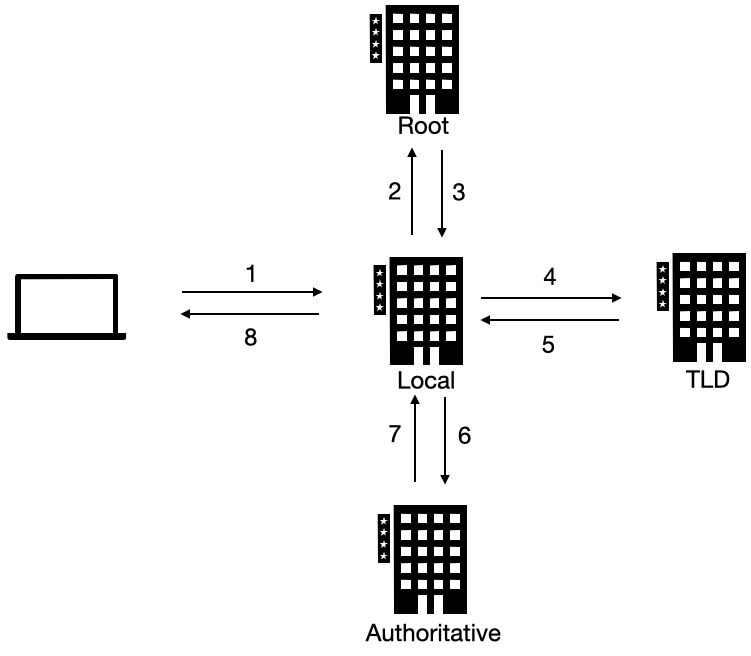
\includegraphics[keepaspectratio, width=12cm, height=9cm]{imagens/10/10 - modelo iterativo.png}
\caption{Modelo Iterativo \\}
\label{Modelo Iterativo}
\end{figure}



\hypertarget{recursivo}{%
\subsubsection{Recursivo}\label{recursivo}}

No modelo recursivo, mostrado na Figura \ref{Modelo Recursivo}, a sequência de \emph{requests} ocorrem em cadeia
entre os servidores:

\begin{enumerate}
\def\labelenumi{\arabic{enumi}.}
\tightlist
\item
  Usuário: \emph{request} para o \emph{local server}
\item
  \emph{Local server}: \emph{request} para \emph{root server}
\item
  \emph{Root server}: \emph{request} para TLD \emph{server}
\item
  TLD \emph{server}: \emph{request} para \emph{Authorative server}
\item
  TLD \emph{server}: \emph{response} do \emph{Authorative server}
\item
  \emph{Root server}: \emph{response} do TLD \emph{server}
\item
  \emph{Local server}: \emph{response} do \emph{root server}
\item
  Usuário: \emph{response} do \emph{local server}
\end{enumerate}


\begin{figure}[H]
\centering
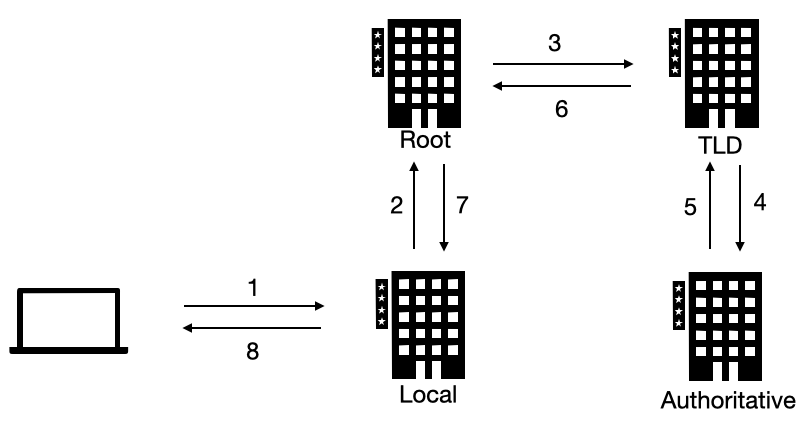
\includegraphics[keepaspectratio, width=12cm, height=9cm]{imagens/10/10 - modelo recursivo.png}
\caption{Modelo Recursivo \\}
\label{Modelo Recursivo}
\end{figure}



\hypertarget{dns-caching}{%
\section{DNS caching}\label{dns-caching}}

Nos dois modelos apresentados anteriormente, foi necessário 8 DNS
\emph{query messages} para a execução do serviço de tradução de
\emph{hostname} para IP \emph{address} (esse número pode ser maior, caso
houver \emph{Authorative servers} intermediários). Porém, de forma a
minimizar os impactos de tantas requisições, o \emph{local server}
utiliza um sistema de armazenamento temporário (pois o mapeamento entre
\emph{hostname} e IP \emph{address} não é permanente, alterando-se com o
tempo) da tradução, fazendo com o número de DNS \emph{query messages}
caia para apenas 2, o \emph{request} e o \emph{response} entre o usuário
e o \emph{local server}.

\hypertarget{vulnerabilidades}{%
\section{Vulnerabilidades}\label{vulnerabilidades}}

O DNS pode ser visto como um multiplicador de requisições, transformando
1, originada do usuário, em 8, que ocorrem entre os servidores do DNS,
algo que o torna especialmente vulnerável à ataques do tipo
\emph{Distributed Denial of Service} (DDoS). Para evitar tal fato, vem
sendo desenvolvido o DNSSEC (DNS \emph{Security Extensions}), uma versão
de segurança do DNS.

\hypertarget{resource-records}{%
\section{Resource Records}\label{resource-records}}

O DNS é um banco de dados distribuídos que armazena uma tupla de 4
elementos, \emph{Name}, \emph{Value}, \emph{Type} e \emph{time to live}
(TTL), o qual é utilizado para prover, entre outros, o mapeamento do
\emph{hostname} para IP \emph{address}. O dado armazenado em cada um dos
2 primeiros elementos citados da tupla variam conforme o \emph{type}. O
último elemento especifica quando o \emph{resource record} deve ser
removido do \emph{cache}.

A seguir será mostrado os dados contidos em \emph{Name} e \emph{Value}
para cada caso de \emph{Type} (os exemplos mostrados não contém o TTL).

\texttt{tupla\ =\ (name,\ value,\ type,\ ttl)}

\emph{Type} A\\
\emph{Name} = \emph{hostname}, \emph{Value} = IP \emph{address}\\
Tupla: \texttt{(relay1.bar.foo.com,\ 145.37.93.126,\ A)}

\emph{Type} NS\\
\emph{Name} = \emph{domain}, \emph{Value} = \emph{Authorative hostname
server}\\
Tupla: \texttt{(foo.com,\ dns.foo.com,\ NS)}

\emph{Type CNAME}\\
\emph{Name} = apelido (\emph{alias}) para \emph{hostname} , \emph{Value}
= \emph{hostname}\\
Tupla: \texttt{(foo.com,\ relay1.bar.foo.com,\ CNAME)}

\emph{Type MX}\\
\emph{Name} = apelido (\emph{alias}) do \emph{mail hostname},
\emph{Value} = \emph{mail hostname}\\
Tupla: \texttt{(foo.com,\ mail.bar.foo.com,\ MX)}


\hypertarget{dns-messages}{%
\subsubsection{\texorpdfstring{DNS
\emph{Messages}}{DNS Messages}}\label{dns-messages}}



O formato da mensagem DNS é mostrado na Figura \ref{Formato do DNS message}, segue a seguinte
estrutura:

\begin{figure}[H]
\centering
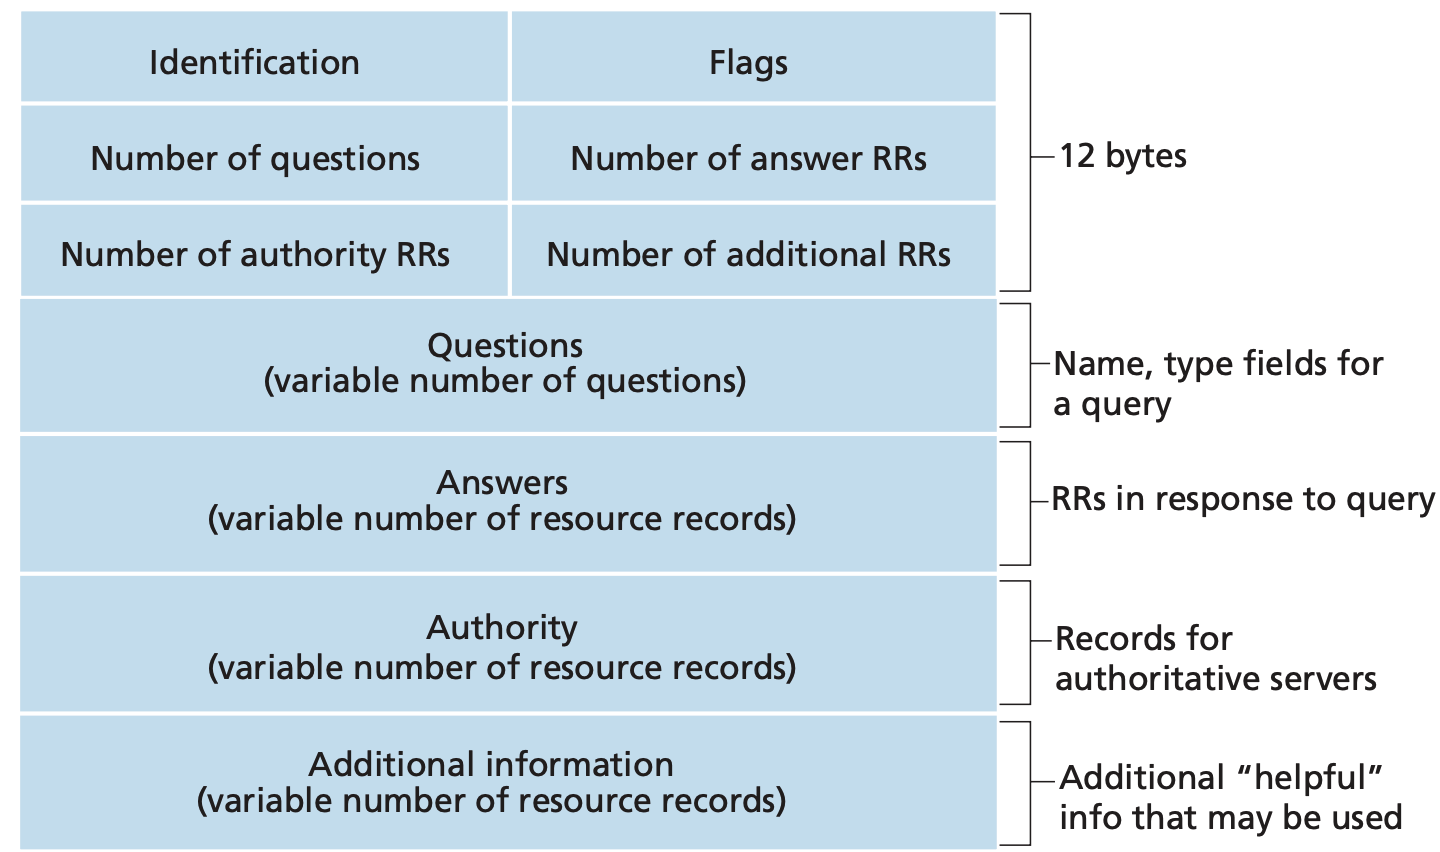
\includegraphics[keepaspectratio, width=12cm, height=9cm]{imagens/10/10 - DNS message format.png}
\caption{Formato do DNS message\\}
\label{Formato do DNS message}
\end{figure}


\begin{enumerate}
\def\labelenumi{\arabic{enumi}.}
\tightlist
\item
  Identificador: número de 16 bits que identifica a \emph{query}
\item
  Flags: cada flag é um indicador de 1 bit, no qual:\\
  2.1. \emph{query}/\emph{reply}: indica se é uma \emph{query} (0) ou um
  \emph{reply} (1)\\
  2.2. \emph{authoritative flag}: indica se o \emph{response} vem de um
  \emph{authorative server}\\
  2.3. \emph{recursion-desire}: indica o desejo do modelo recursão para
  as requisições (como mostrado anteriormente)\\
  2.4. \emph{recursion-available field}: ajustado na resposta, indica se
  o DNS \emph{server} suporta recursão
\item
  \emph{Number fields}: cada campo indica o número de ocorrências de
  cada sessão de dados
\item
  \emph{Questions}: contém informações como: \emph{host address} e
  \emph{name}, para \emph{type} A.
\item
  \emph{Answers}: populado pelo DNS \emph{server}, contém os
  \emph{resource records} para o \emph{hostname} requisitado.
\item
  \emph{Authority}: \emph{records} de \emph{authority servers}
\item
  \emph{Additional information}: contém outras informações
  interessantes.
\end{enumerate}

\hypertarget{adicionando-rr-no-banco-de-dados-dns}{%
\paragraph{Adicionando RR no banco de dados
DNS}\label{adicionando-rr-no-banco-de-dados-dns}}

A verificação (de unicidade) e adição de um novo RR no DNS é feito
através de entidades comerciais chamadas de \emph{registrar}, as quais
são acreditadas pela \emph{Internet Assigned Names and Numbers} (ICANN).
Para a adição, é necessário prover o \emph{domain name}, por exemplo
\texttt{google.com.br}, e o endereço de IP do DNS primário e secundário.

\hypertarget{complementar-4}{%
\section{Complementar}\label{complementar-4}}

\hypertarget{pesquisar-sobre-3}{%
\subsection{Pesquisar Sobre}\label{pesquisar-sobre-3}}

\begin{enumerate}
\def\labelenumi{\arabic{enumi}.}
\tightlist
\item
  https://alexanderell.is/posts/rpc-from-scratch/
\item
  https://datatracker.ietf.org/doc/html/rfc/
\item
  DNS over HTTPS (DoH): https://datatracker.ietf.org/doc/html/rfc8484
\item
  DNS over TLS (DoT): https://datatracker.ietf.org/doc/html/rfc8310
\end{enumerate}